\chapter{Морфизмы и прочие гадости}

По лекции от 14 сентября 2011 года.

\section{Большая куча определений}

\begin{Def}
	$\phi : G_1 \rightarrow G_2$ - гомоморфизм, если выполняются условия:
	\begin{enumerate}
		\item $\phi \left( xy \right) = \phi \left( x \right) \phi \left( y \right)$

		\item $\phi \left( 1 \right) = 1$

		\item $\phi \left( X^{-1} \right) = \phi \left( x \right) ^{-1}$
	\end{enumerate}
\end{Def}

\paragraph{Примечание:} группы $G_1$ и $G_2$ ообще говоря имеют раличные групповые операции и, соответственно, обозначения для них.

\paragraph{Примечание:} из утверждений 1 и 2 следует 3.
\begin{Proof}
	$\phi \left(x x^{-1}\right) = \phi \left( x \right) \phi \left( x^{-1} \right) = \phi \left(x\right) \phi \left(x\right)^{-1} = 1$
\end{Proof}

\paragraph{Примечание:} из утверждений 1 и 3 следует 2.
\begin{Proof}
	$\phi \left(1\right) = \phi \left(x x^{-1}\right) = \phi \left( x \right) \phi \left( x^{-1} \right) = \phi \left(x\right) \phi \left(x\right)^{-1} = 1$
\end{Proof}

\paragraph{Примечание:} образ гомоморфизма не обязательно совпадает со всей группой $G_2$

\begin{Def}
	Мономорфизм - инъективный гомоморфизм. (Различные элементы $G_1$ переводятся в различные элементы $G_2$, или у любого элемента из $G_2$ не более одного прообраза)
\end{Def}

\begin{Def}
	Эпиморфизм - сюръективный гомоморфизм. (Любой элемент $G_2$ является образом элемента из $G_1$)
\end{Def}

\begin{Def}
	Изоморфизм - биективный изоморфизм (мономорфизм и эпиморфизм одновременно)
\end{Def}

\begin{Def}
	Эндоморфизм - гомоморфизм из группы в саму себя
\end{Def}

\begin{Def}
	Атоморфизм - изоморфизм и эндоморфизм одновременно
\end{Def}

\begin{Def}
	$Aut(G)$ - множество всех автоморфизмов.
\end{Def}

\begin{figure}[h]
	\begin{minipage}[h]{0.4\linewidth}
		\noindent\center{
			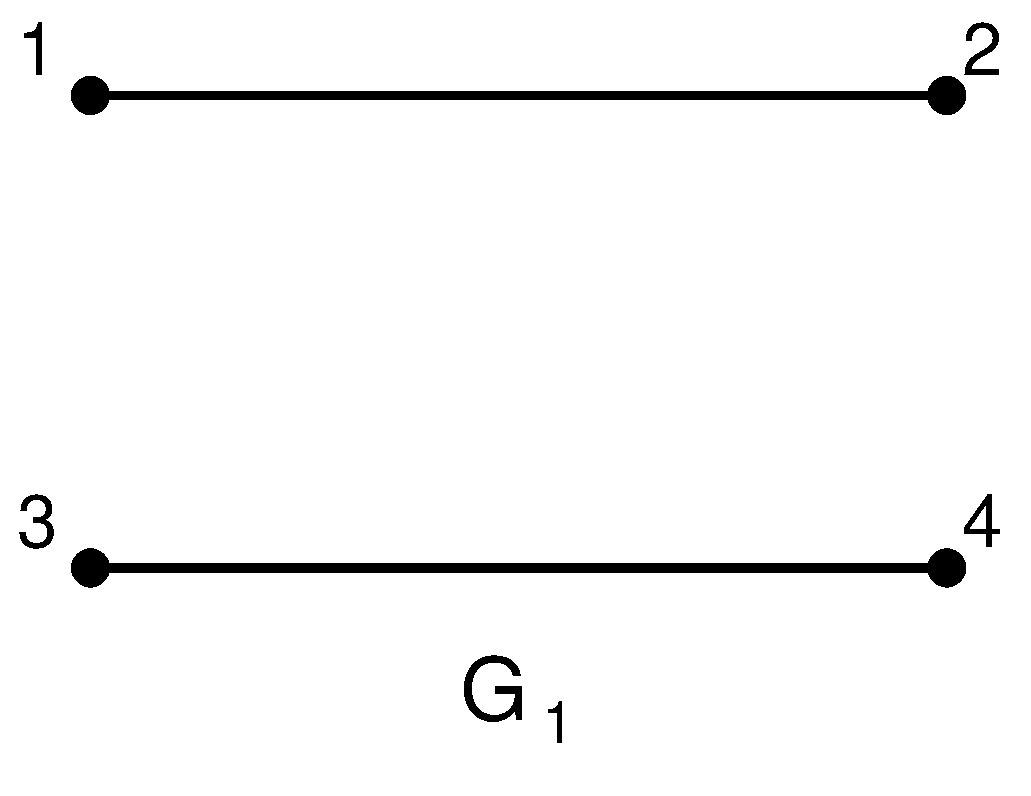
\includegraphics[width=0.8\linewidth]{graph1}
		}
	\end{minipage}
	\hfill
	\begin{minipage}[h]{0.4\linewidth}
		\noindent\center{
			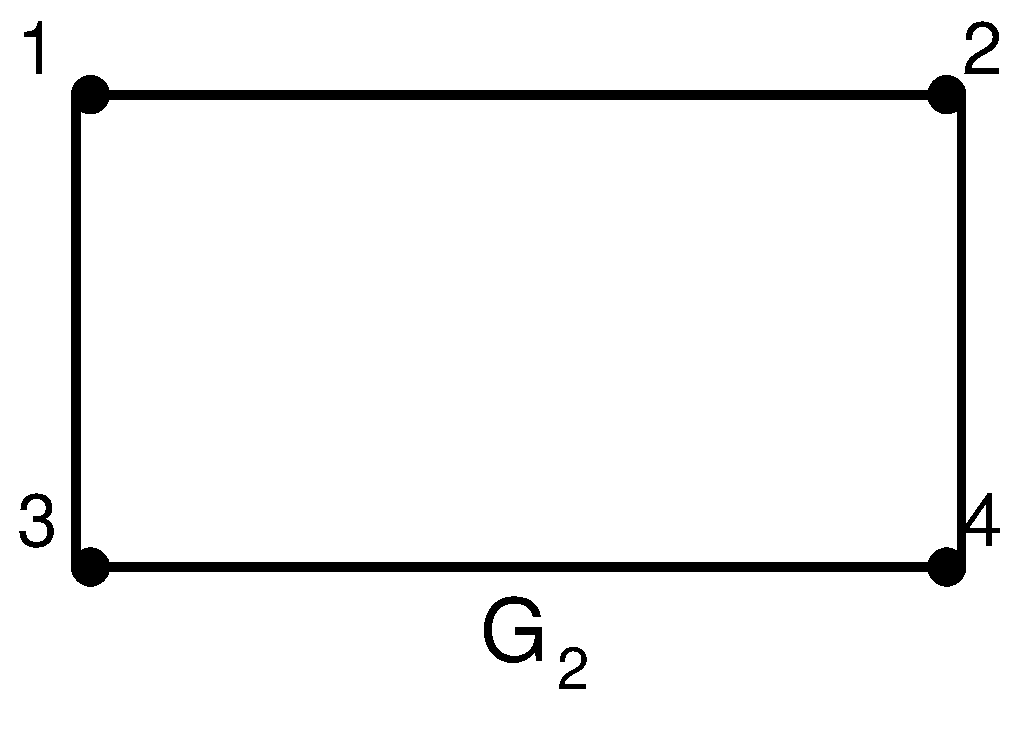
\includegraphics[width=0.8\linewidth]{graph2}
		}	\end{minipage}
	\label{pic::graphs}
\end{figure}

\paragraph{Задача} Доказать, что $Aut(G_1) \cong Aut(G_2)$ (см. рис. \ref{pic::graphs})

\begin{Solution}
\begin{figure}[h]
	\noindent\center{
		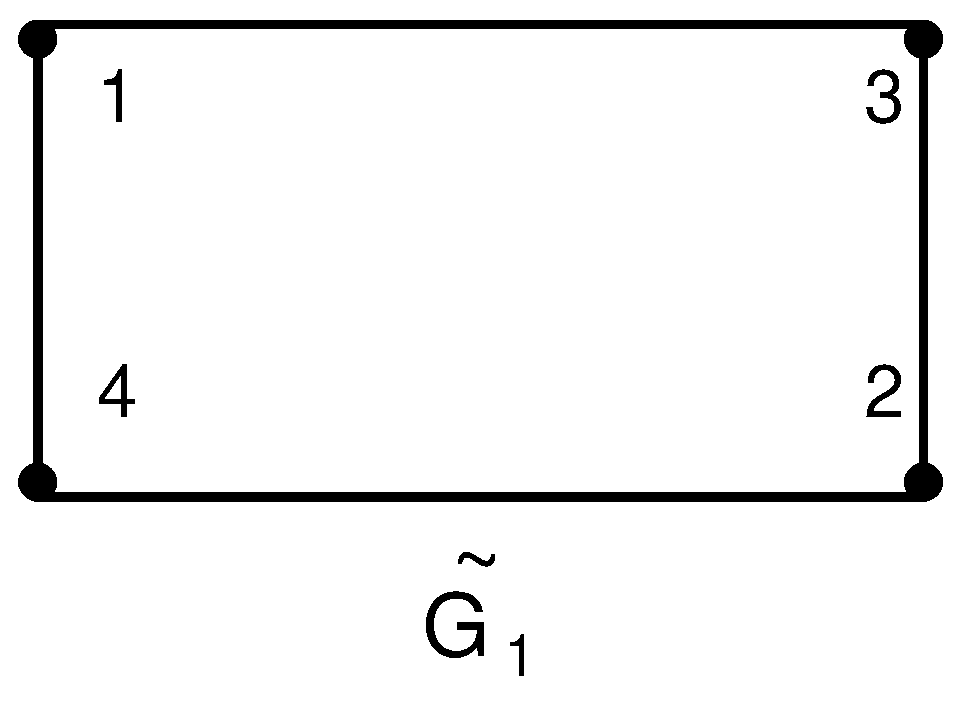
\includegraphics[width=0.4\linewidth]{tilde_graph}
	}
	\label{pic::tilde_graph}
\end{figure}

	Заменим наличие ребер их отсутсвием в графе $G_1$ получаем граф $\tilde {G_1}$, изображенный на рисунке \ref{pic::tilde_graph}, оба графа эквивалентны, так как по одному однозначно восстанавливается другой, а кроме того, не трудно увидеть, что $\tilde G_1$ получается из $G_2$ простой перенумерацией вершин, а значит и группы автоморфизмов графов изоморфны.
\end{Solution}

\paragraph{Обозначение:}
Мономорфизм $G_1 \rightarrowtail G_2$

Эпиморфизм $G_1 \twoheadrightarrow G_2$
